\section{Evaluation}
\label{ch:eval}

In this chapter, we conduct evaluations to our collected data.
The data is collected from 21 subjects, and 189 clickstream data are collected in total. 
Each clickstream contains action-level data with a stay duration
of a specific page, for instance, we still collect an URL as a step of clickstream 
if a participant uses back button rollback to a previous visited page without requesting server. 
A clickstream also has a subjective difficulty score from questionaire (shown in Appendix \ref{appendix:b}) 
after the completion of each task.

\subsection{Subjective Task Difficulty}

This section discusses the subjective task difficulty qualitatively and quantitatively.
Figure \ref{fig:difficulty} illustrates a normalized (raw scores are listed in 
Appendix \ref{appendix:c} Table \ref{table:diff}) subjective difficulty score 
with respect to all tasks.

\begin{figure}[H]
    \centering
    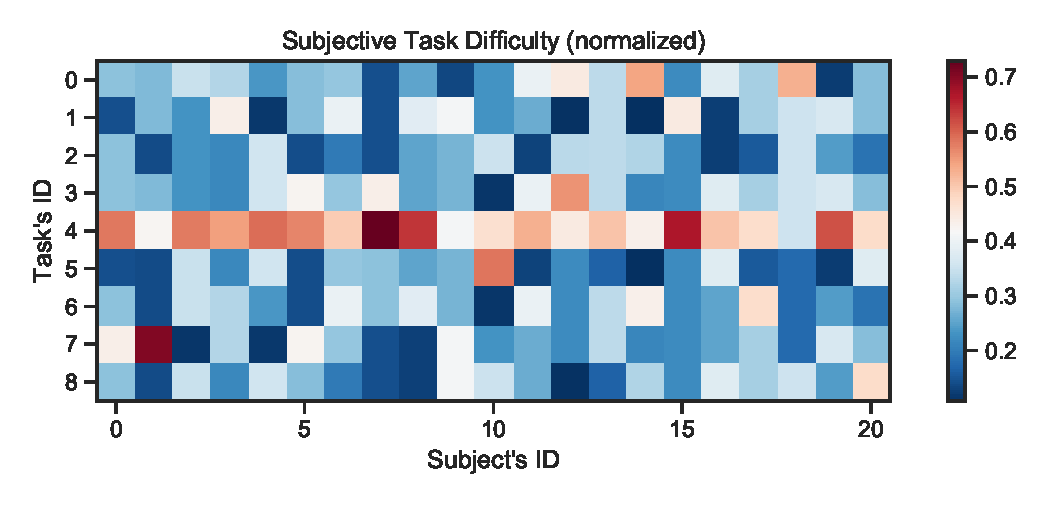
\includegraphics[width=0.7\textwidth]{figures/difficulty}
    \caption{Subjective difficulty score: each column indicates an individual subject and
    each row indicates a browsing task. Tasks from 0 to 8 represent Amazon Goal Oriented Task,
    Amazon Fuzzy Task, Amazon Exploring Task; Medium Goal Oriented Task, Medium Fuzzy Task,
    Medium Exploring Task, Dribbble Goal Oriented Task, Dribbble Fuzzy Task and Dribbble Exploring Task
    respectively.
    From this heat map, we clearly observes Medium Fuzzy Task is the most difficulty task
    according to the subjects voted subjective difficulty, a significant test confirmed this observation.
    Further, Mann-Whitney U significant test justifies our result.}
    \label{fig:difficulty}
\end{figure}

To generalize the task difficulty, the null hypothesis ($H_0$): the difficulty of fuzzy task is not greater
than exploring task and alternative hypothesis ($H_1$): the difficulty of fuzzy task is greater than
exploring task. We conduct non-parametric one-tailed Mann-Whitney U test \cite{mann1947test}, 
under null hypothesis, $p=2.54\times 10^{-5} < 0.05$, reject $H_0$.
Similarly, we compare difficulty score on goal oriented task and exploring task (with corresponding hypothesis, 
$p=0.00534 < 0.05$), difficulty score on fuzzy task and goal oriented task (with corresponding hypothesis, 
$p=0.0145 < 0.05$), all rejects $H_0$. Therefore we concludes the task difficulty is ordered
as follows: \emph{difficulty of fuzzy task $>$ difficulty of goal oriented task $>$ difficulty of exploring task},
which means exploring tasks have lower effort in clickstream, and effort of doing fuzzy task gains highest effort.

\subsection{Browsing Behavior Classification}

As discussed in Section \ref{sec:task-design}, we described three type of browsing behavior. 
In this section, we provides two type of evaluations to interpret the browsing behavior classification.

First, we evaluate the indication of general features browsing behavior,
features including difficulty of task, number of actions in a clickstream as well as the total stay duration in a clickstream.
Then we implements our action path model by using the action-level clickstream data and stay duration of each page,
which was described in Section \ref{sec:recurrent-unit} and \ref{sec:mark-interpretation}.

\subsubsection{Interpretation based on General Features}
\label{sec:inter-general-feature}

% \begin{figure}[H]
%     \centering
%     \includegraphics[width=0.49\textwidth]{figures/amazon-general}
%     \includegraphics[width=0.49\textwidth]{figures/medium-general}
%     \includegraphics[width=0.49\textwidth]{figures/dribbble-general}
%     \caption{XXXXX}
%     \label{fig:general}
% \end{figure}

\begin{figure}[H]
    \centering
    \includegraphics[width=0.25\textwidth]{figures/tsne-amazon}
    \includegraphics[width=0.25\textwidth]{figures/2d-eff-dur-amazon}
    \includegraphics[width=0.25\textwidth]{figures/2d-eff-len-amazon}
    \includegraphics[width=0.25\textwidth]{figures/2d-len-dur-amazon}
    \caption{TODO:}
    \label{fig:general-amazon}
\end{figure}

TODO: table of classification report

more U-test, feature importance.

\subsubsection{Intepretation based on Action Path}
\label{sec:inter-action-path}

To use full capacity of our data, this section uses the entire clickstream and its corresponding
page-level stay time duration as input, three ending mark (<EOA\_GOAL>, <EOA\_FUZZY>, and <EOA\_EXPLORE>) 
as classification outputs, and then implements a single GRU layer action path model 
to classify the three type of tasks.

Our training parameters are: 
The GRU latent dimension is 10, training process feeds 151 clickstreams and 
propagates 500 epochs with batch size of 32.
In the end of training, we use Adam optimizer, evaluate on 38 clickstreams and 
archieved 100\% accuracy on our validation set.

The validation loss during the training is as shown in Figure \ref{fig:class-loss}.

\begin{figure}[H]
    \centering
    \includegraphics[width=0.75\textwidth]{figures/class-loss}
    \caption{Categorical Cross-Entropy Validation loss curve while 500 epoches. 
    The curves indicates the training process is not an overfitting since the loss is not increasing.}
    \label{fig:class-loss}
\end{figure}

One can observed that the training process is not an overfit, and the validation loss is 
still not increase after 500 epoches, thus, single GRU layer action path model 
remains a large expressive performance (100\% of three class classification in this dataset) 
when we have more data.

In addition, the action path model feeds the entire clickstream and time duration as inputs, 
therfore the entire clickstream contains informations regarding the number of visit actions
as well as completion effeciency and etc. Consequently, we conclude that the model works
perfectly on the classification of three different browsing behavior. Since our experiment is
only designed for three type of behavior, and the learning curve
shows the model still has capacity to classify more precise categories of browsing behavior,
perform a future investigation may be significance.

\subsection{Optimal Action Path Context}

This section we evaluates our model with limited action path context, where the feeding action path
are limited based on a split ratio. For instance, if a split ratio is 0.8 then we feed 80\% of 
an action path into the model, then predict the rest of 20\% actions. Figure \ref{} illustrates
the best accuracy we archieved for when use different split ratio.

\begin{figure}[H]
    \centering
    \includegraphics[width=0.7\textwidth]{figures/acc}
    \caption{TODO:}
    \label{fig:acc}
\end{figure}

\begin{figure}[H]
    \centering
    \includegraphics[width=0.45\textwidth]{figures/loss1}
    \includegraphics[width=0.45\textwidth]{figures/loss2}
    \caption{TODO:}
    \label{fig:loss}
\end{figure}


\subsection{Action Path Visualization}

This section visualizes the actual action path of users and discusses the behavior qualitatively.
Note that we collected 189 clickstream in total, which is not possible to illustrate all of them
in the thesis, we selected three typical clickstreams to discuss and provided a visualization tool
to help readers to explore them.

\subsubsection{Individual Common Patterns}

\begin{figure}[H]
    \centering
    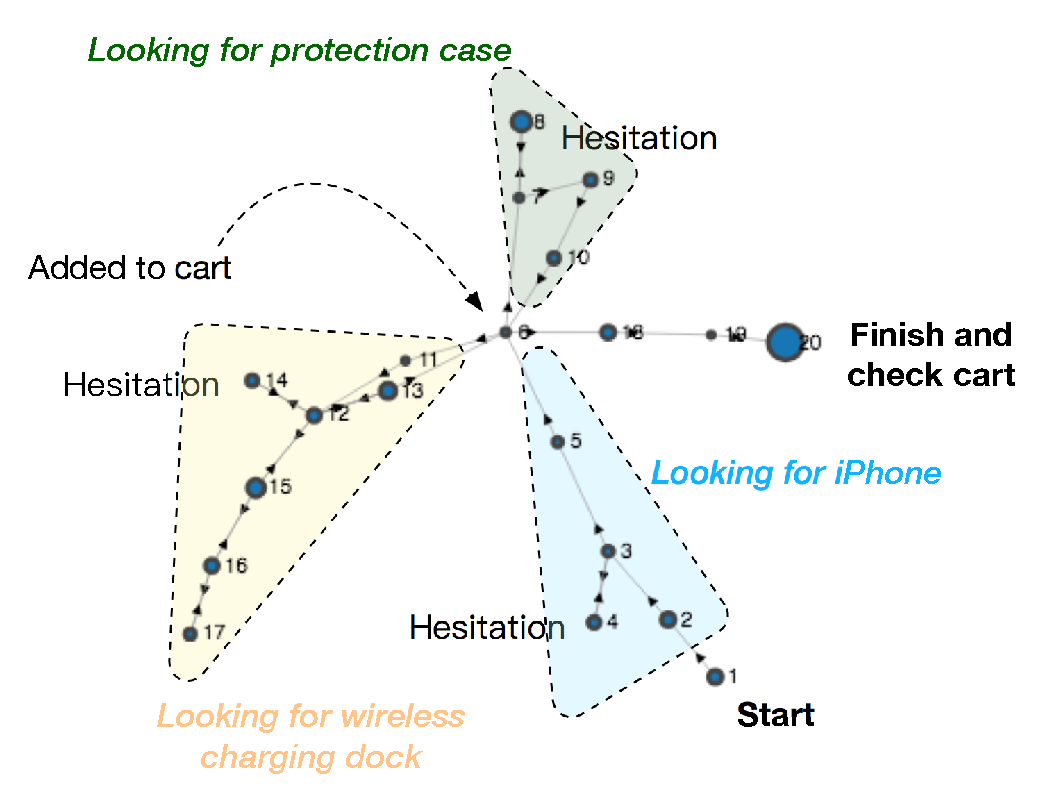
\includegraphics[width=0.45\textwidth]{figures/vis-goal1}
    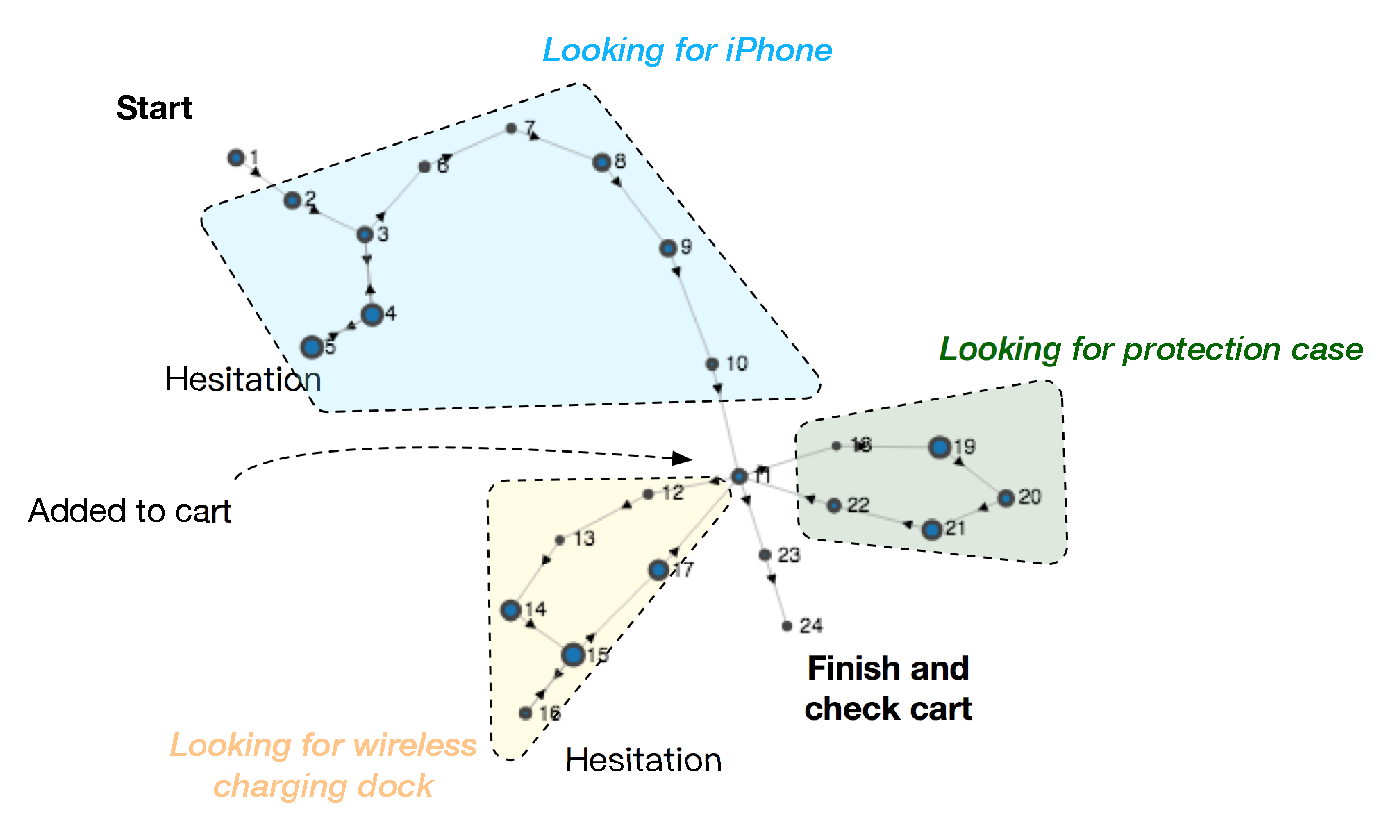
\includegraphics[width=0.45\textwidth]{figures/vis-goal2}
    \caption{TODO:}
    \label{fig:vis-goal}
\end{figure}


\begin{figure}[H]
    \centering
    \includegraphics[width=0.45\textwidth]{figures/vis-fuzzy-explore1}
    \includegraphics[width=0.45\textwidth]{figures/vis-fuzzy-explore2}
    \caption{TODO:}
    \label{fig:vis-fuzzy-explore}
\end{figure}

\subsubsection{Cross-user Overlap Patterns}

\begin{figure}[H]
    \centering
    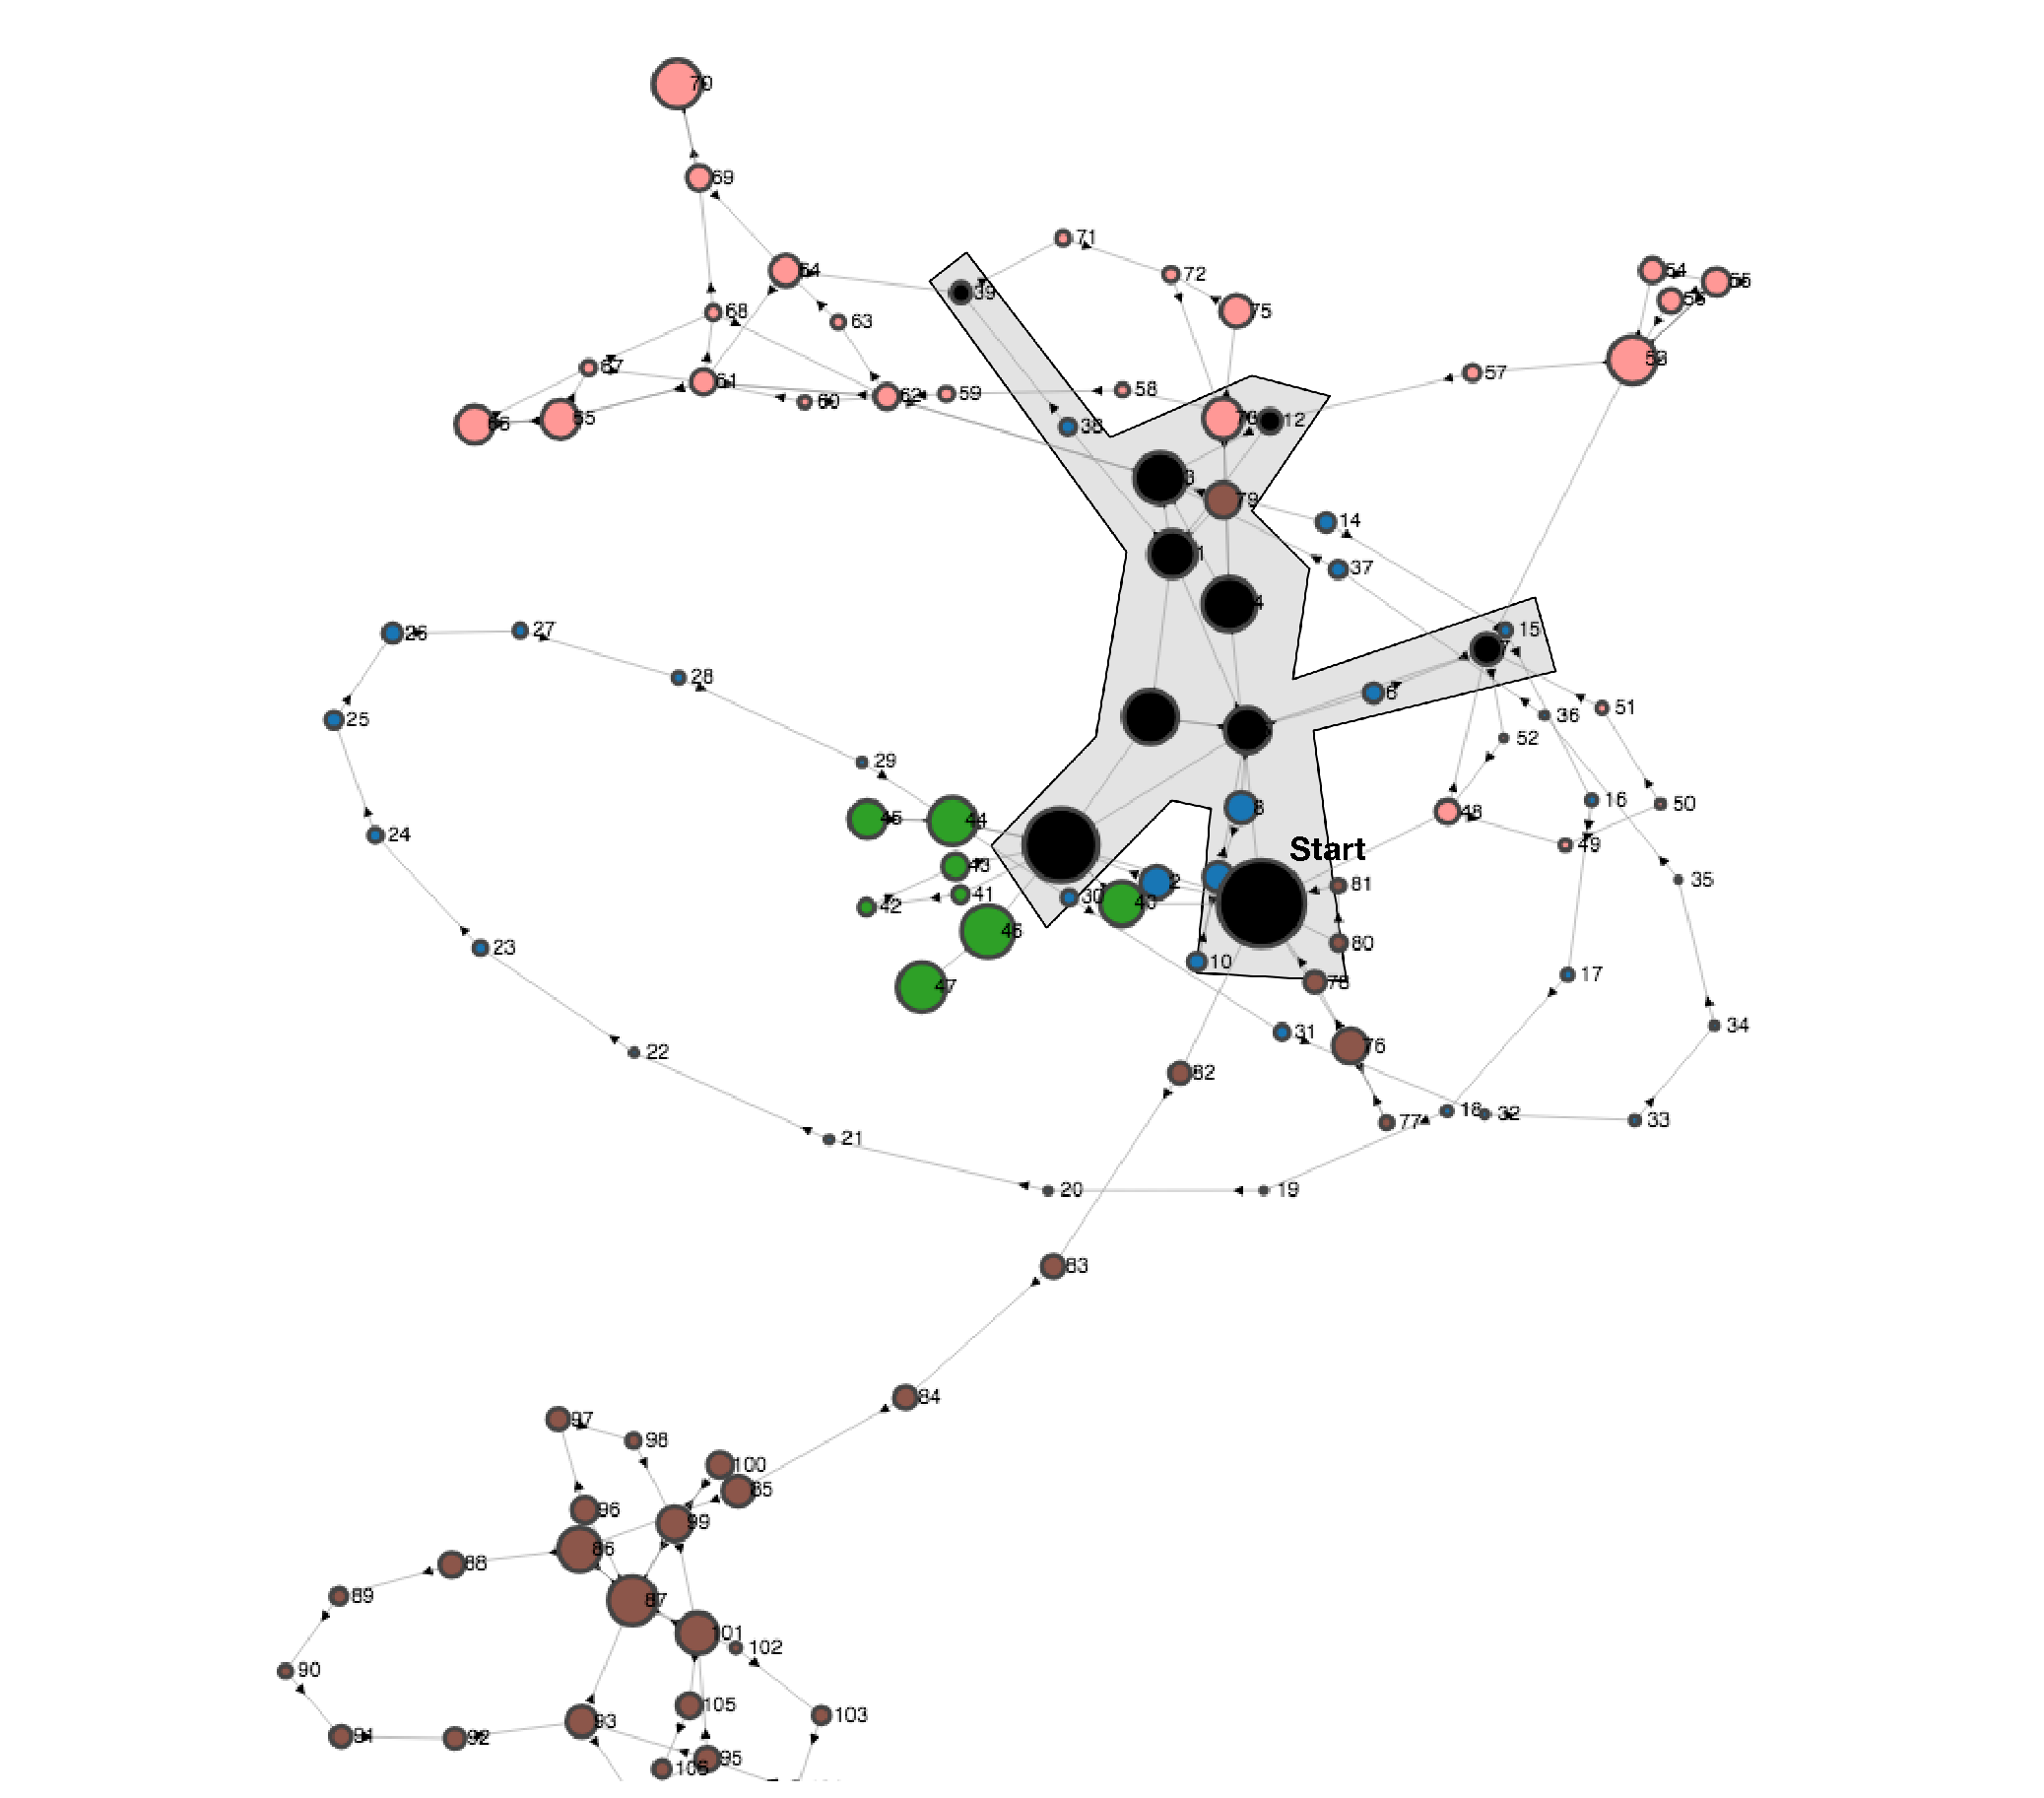
\includegraphics[width=0.45\textwidth]{figures/overlap1}
    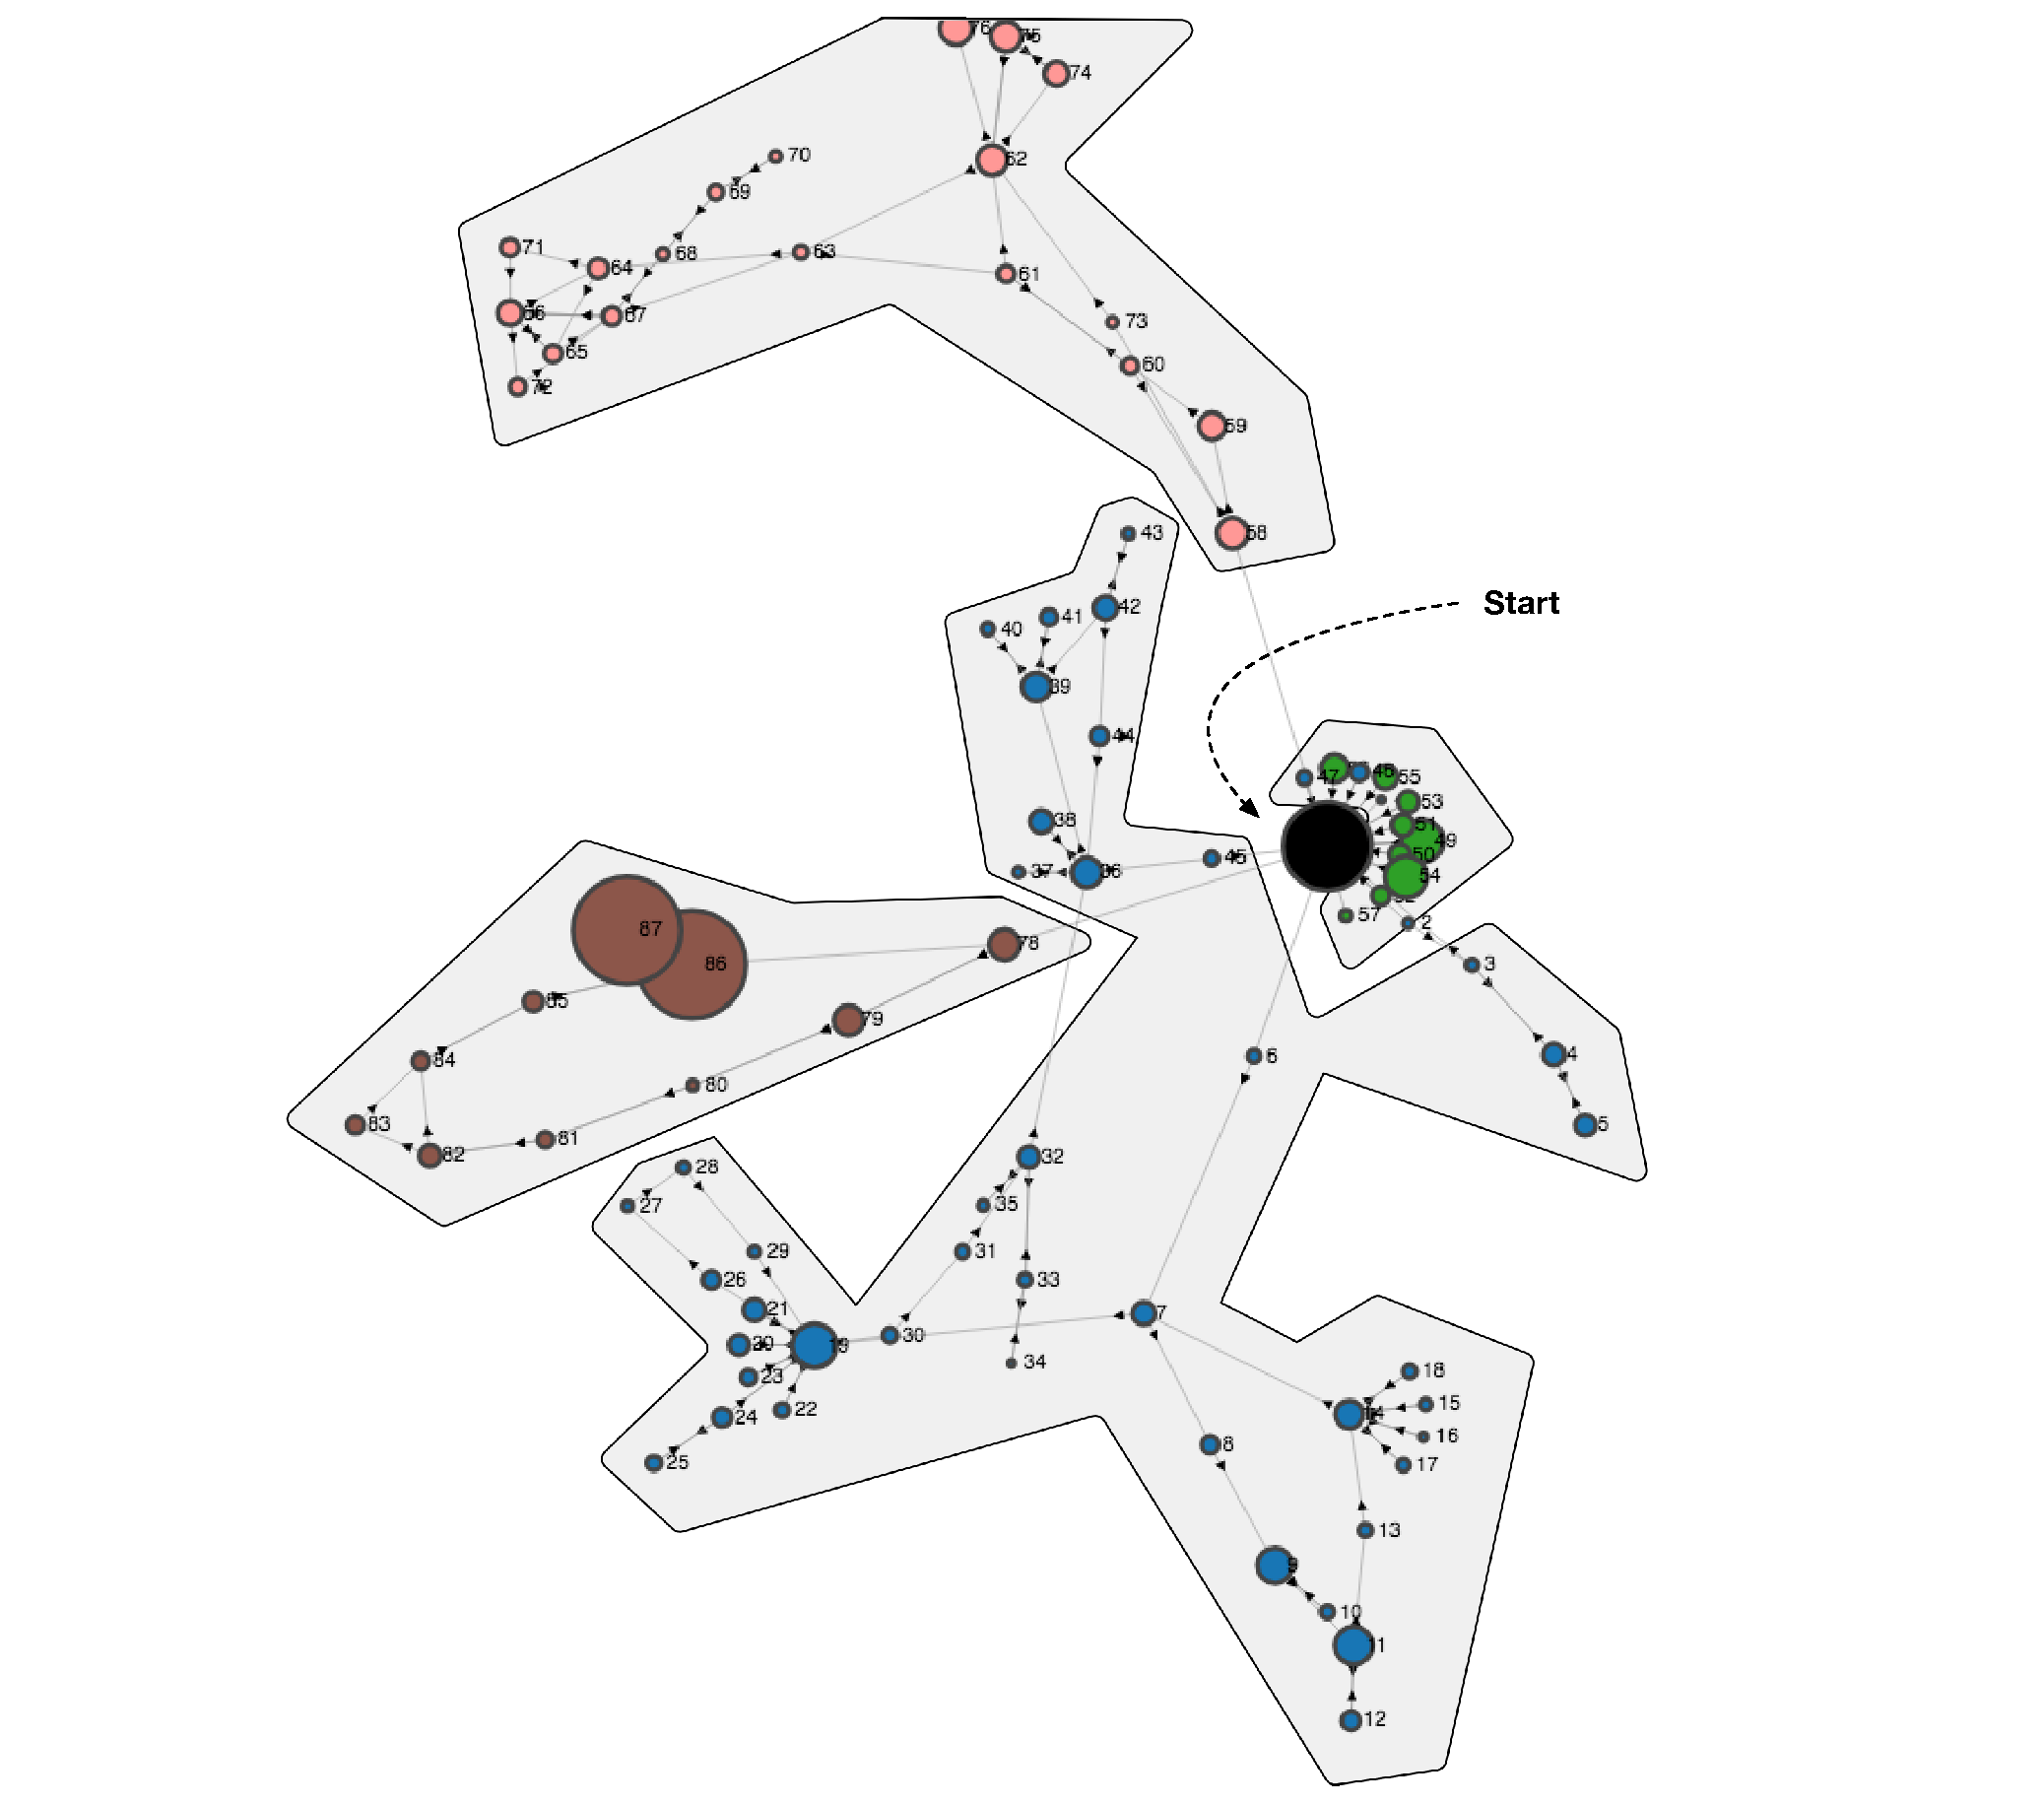
\includegraphics[width=0.45\textwidth]{figures/overlap2}
    \caption{TODO:}
    \label{fig:overlap}
\end{figure}



\cleardoublepage